% Created 2026-04-23 Thu 12:09
% Intended LaTeX compiler: lualatex
\DocumentMetadata{lang = en-US,pdfversion = 2.0,pdfstandard = ua-2,tagging = on,tagging-setup = {math/setup=mathml-SE},}
\documentclass[11pt]{article}
\usepackage{amsmath}
\usepackage{fontspec}
\usepackage{graphicx}
\usepackage{longtable}
\usepackage{wrapfig}
\usepackage{rotating}
\usepackage[normalem]{ulem}
\usepackage{capt-of}
\usepackage{hyperref}
\usepackage[margin=1in]{geometry}
\usepackage{fontspec}
\usepackage{verbatim, multicol, tabularx,}
\usepackage{amsmath, amsthm, amssymb, stmaryrd, latexsym, bm, listings, qtree}
\usepackage{framed}
\usepackage{xcolor,colortbl}
\usepackage{media9}
\usepackage[export]{adjustbox}
\usepackage{algorithm}
\usepackage[noend]{algpseudocode}
\usepackage{tikz,pgfplots}
\usetikzlibrary{shapes.geometric}
\let\oldquote=\quote
\let\endoldquote=\endquote
\colorlet{shadecolor}{cyan!15}
\renewenvironment{quote}{\begin{shaded*}\begin{oldquote}}{\end{oldquote}\end{shaded*}}
% From https://tex.stackexchange.com/questions/7032/good-way-to-make-textcircled-numbers
\newcommand*\circled[1]{\tikz[baseline=(char.base)]{\node[shape=circle,draw,inner sep=2pt] (char) {#1};}}
\DeclareMathOperator*{\argmin}{arg\!min}
\DeclareMathOperator*{\argmax}{arg\!max}
\lstset{frame=tb, aboveskip=1mm, belowskip=0mm, showstringspaces=false, columns=flexible, basicstyle={\scriptsize\ttfamily}, numbers=left, frame=single, breaklines=true, breakatwhitespace=true}
\hypersetup{colorlinks=true,urlcolor=blue}
\usepackage{tagpdf}
\tagpdfsetup{activate-all}
\tagpdfsetup{math/alt/use}
\usepackage{polyglossia}
\setdefaultlanguage[variant=en-US]{english}
\author{Christopher Simpkins}
\date{Kennesaw State University}
\title{Artlificial Intelligence\\\medskip
\large Planning}
\hypersetup{
 pdfauthor={Christopher Simpkins},
 pdftitle={Artlificial Intelligence},
 pdfkeywords={},
 pdfsubject={Artlificial Intelligence Planning},
 pdfcreator={Emacs 30.2 (Org mode 9.7.11)}, 
 pdflang={English}}
\begin{document}

\maketitle
\section{Classical Planning}
\label{sec:org2774430}

Classical planning is the task of finding a sequence of actions to accomplish a goal in a discrete, deterministic, static, fully observable environment.  Two previous approaches:

\begin{itemize}
\item Graph search, e.g., \(A^*\)
\item Hybrid propositional logical agent
\end{itemize}

Two limitations:

\begin{itemize}
\item Require ad-hoc heuristics
\item Require explicit representation of exponentially large state space.
\end{itemize}

Planning Domain Definition Language solves these problems using a factored representation based on first-order logic.

\begin{itemize}
\item A \textbf{state} is a conjunction of ground atomic fluents -- single predicates containing no variables.

\begin{itemize}
\item \(At(Truck_1,Melbourne)\) is a ground atomic fluent, \(At(t_1, from)\) is not.
\end{itemize}

\item PDDL uses \textbf{database semantics}, or the \textbf{closed-world assumption}: any fluents not mentioned are false, and unique names represent distinct objects.
\end{itemize}
\section{Planning Domain Definition Language (PDDL)}
\label{sec:orgae39039}

Action schema is a family of ground actions.

\begin{itemize}
\item Action name and list of variables
\item Precondition: conjunction of literals

\begin{itemize}
\item Action \(a\) is \textbf{applicable} in state \(s\) if \(s \models a.precondition\)
\end{itemize}

\item Effect: conjunction of literals

\begin{itemize}
\item \textbf{Result} of executing action \(a\) in state \(s\) is \(s'\) is applying delete list and add list to \(s\):

\begin{itemize}
\item \(DEL(a)\), delete list: remove negative literals in action's effects.
\item \(ADD(a)\), add list: add positive literals in action's effects.
\end{itemize}
\end{itemize}
\end{itemize}


Action schema:
\vspace{-.25in}
\begin{align*}
& Action(Fly(p,from,to),\\
& \hspace{.1in} PRECOND:At(p,from) \land Plane(p) \land Airport(from) \land Airport(to)\\
& \hspace{.1in} EFFECT: \neg At(p,from) \land At(p,to))
\end{align*}
\vspace{-.25in}

Ground (variable-free) action:

\vspace{-.25in}
\begin{align*}
& Action(Fly(P_1,SFO,JFK), \\
& \hspace{.1in} PRECOND:At(P_1,SFO) \land Plane(P_1) \land Airport(SFO) \land Airport(JFK) \\
& \hspace{.1in} EFFECT: \neg At(P_1,SFO) \land At(P_1,JFK))
\end{align*}
\vspace{-.25in}
\section{Air Cargo Transport}
\label{sec:org1bc3025}


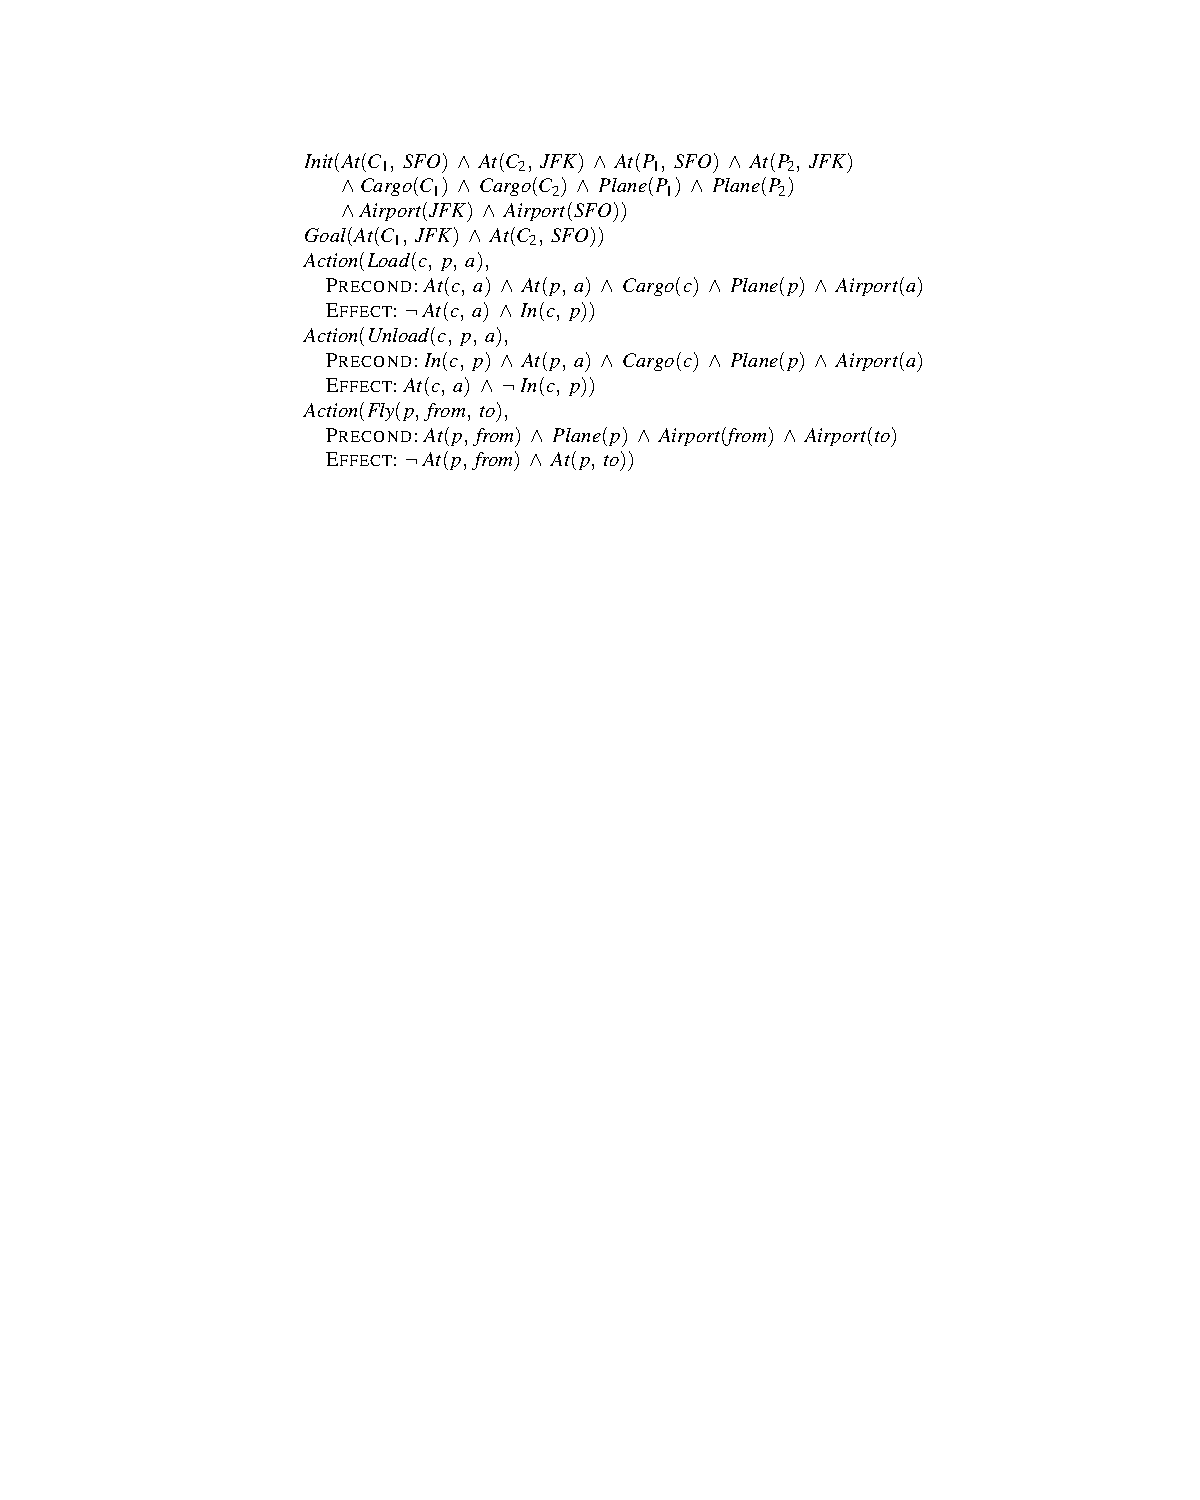
\includegraphics[alt={aima fig 11_01 pddl air cargo},height=2.8in]{aima-fig-11_01-pddl-air-cargo.pdf}
\section{Blocks World}
\label{sec:orged8f0a5}


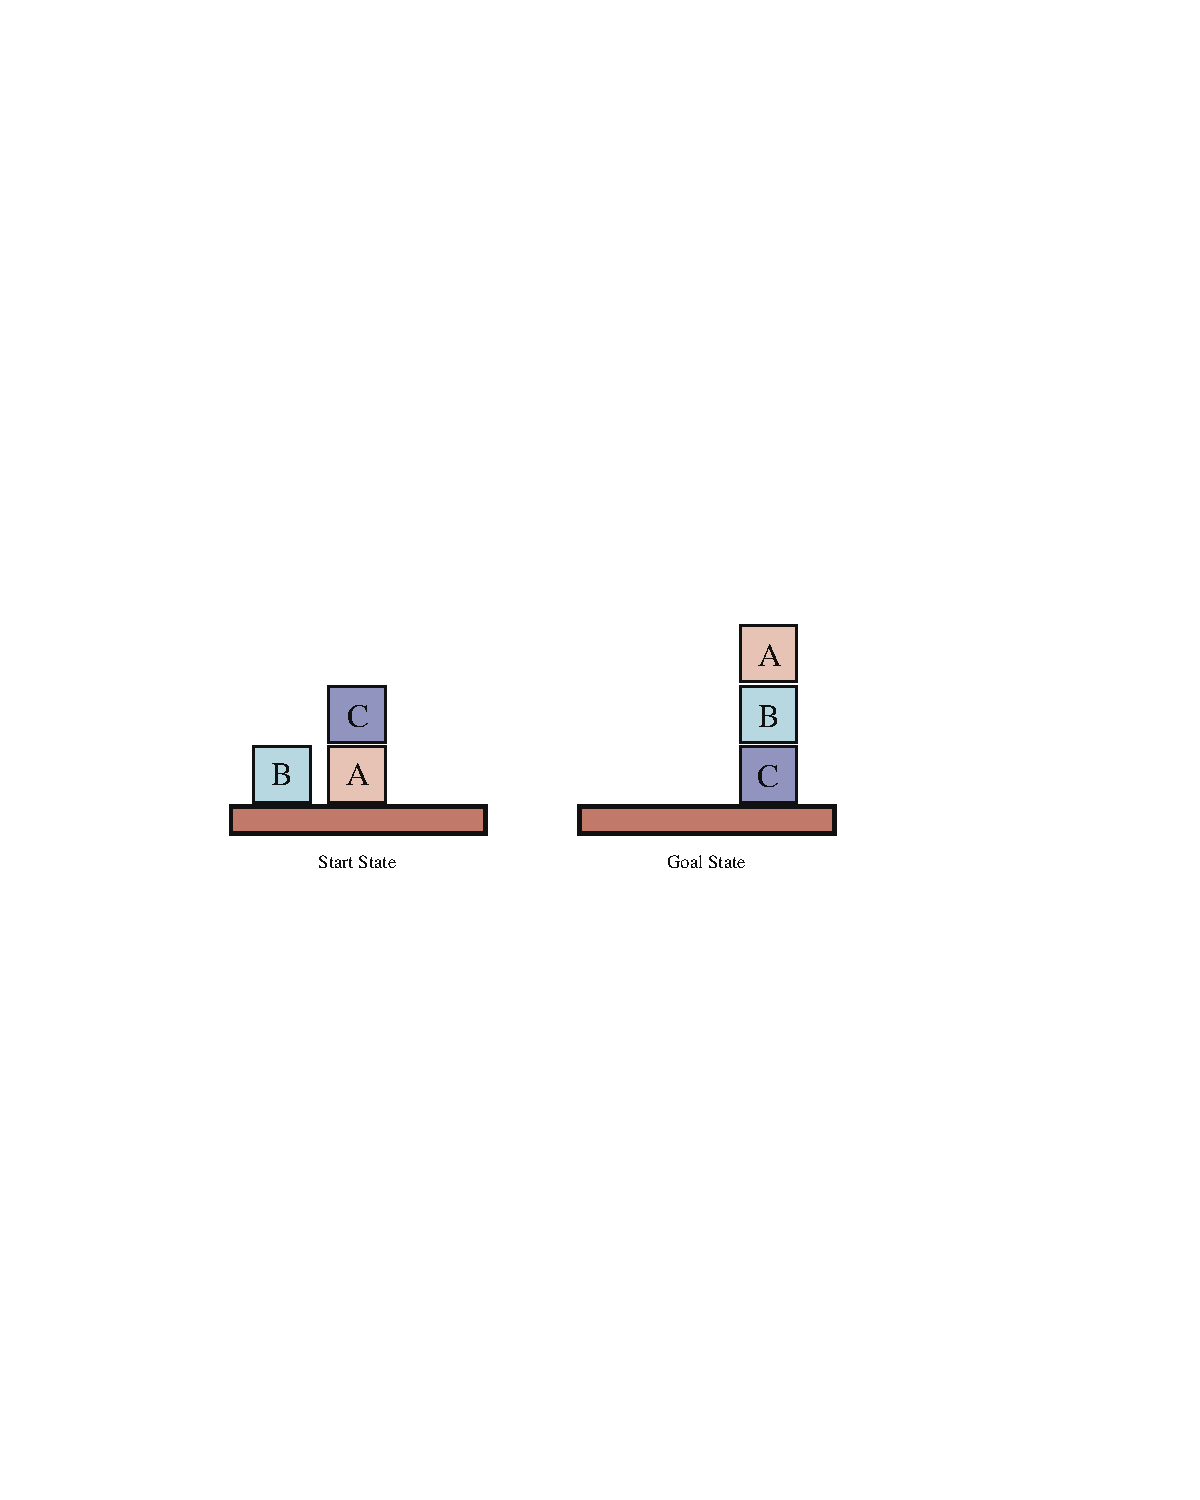
\includegraphics[alt={aima fig 11_03 blocks world diagram},height=2.8in]{aima-fig-11_03-blocks-world-diagram.pdf}
\section{Blocks World PDDL}
\label{sec:orgab0585c}


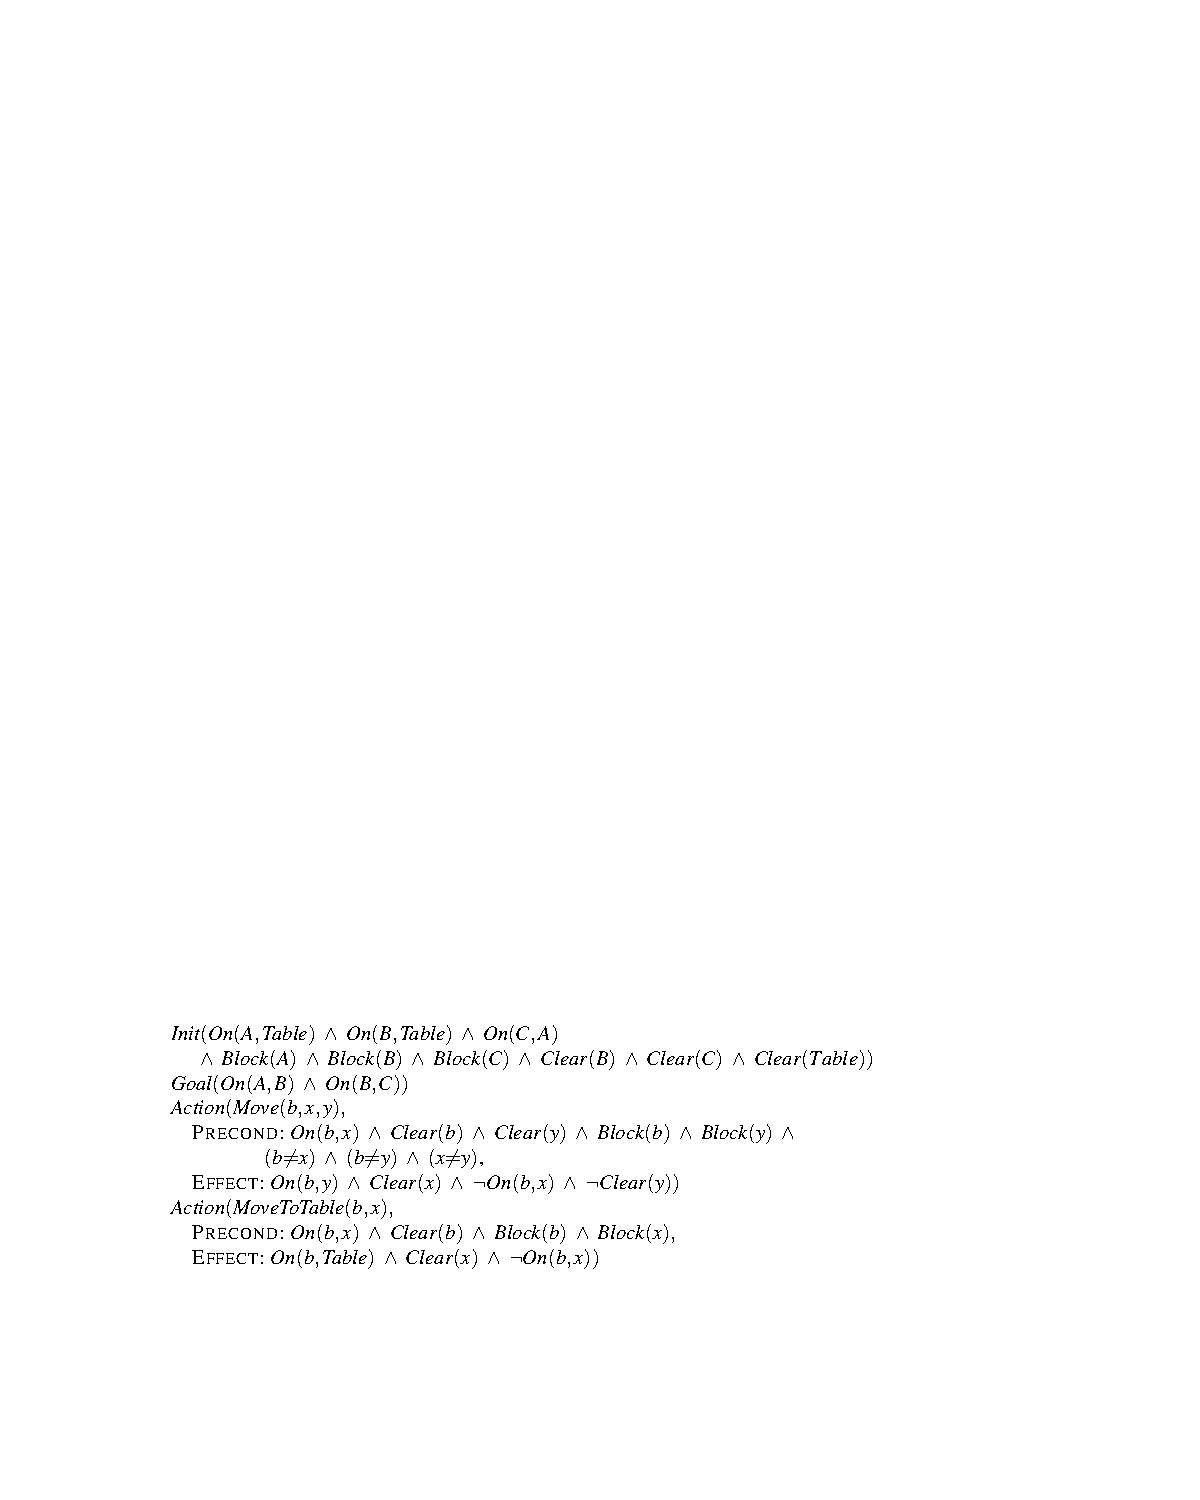
\includegraphics[alt={aima fig 11_04 pddl blocks world},height=2.8in]{aima-fig-11_04-pddl-blocks-world.pdf}
\section{Classical Planning Algorithms}
\label{sec:orgda71617}

\begin{itemize}
\item Forward state space search
\item Backward state space search
\item SATPlan -- boolean satisfiability planning

\begin{itemize}
\item Translate PDDL into propositional form, use a SAT solver
\end{itemize}

\item Graphplan

\begin{itemize}
\item Encode constraints related to preconditions and effects in a \textbf{planning graph}.
\end{itemize}

\item Situation calculus
\item Constraint satisfaction
\item Partial-order planning

\begin{itemize}
\item \(Remove(Spare,Trunk)\) and \(Remove(Flat,Axle)\) must come before \(PutOn(Spare,Axle)\), but removals can happen in any order.
\end{itemize}
\end{itemize}
\section{Forward and Backward State Space Planning}
\label{sec:orgc6c00e9}

\begin{itemize}
\item Forward search: unify current state against preconditions of each action schema -- \textbf{applicable} actions.

\item Backward search: unify goal states against effects of action schemas -- \textbf{relevant} actions.
\end{itemize}


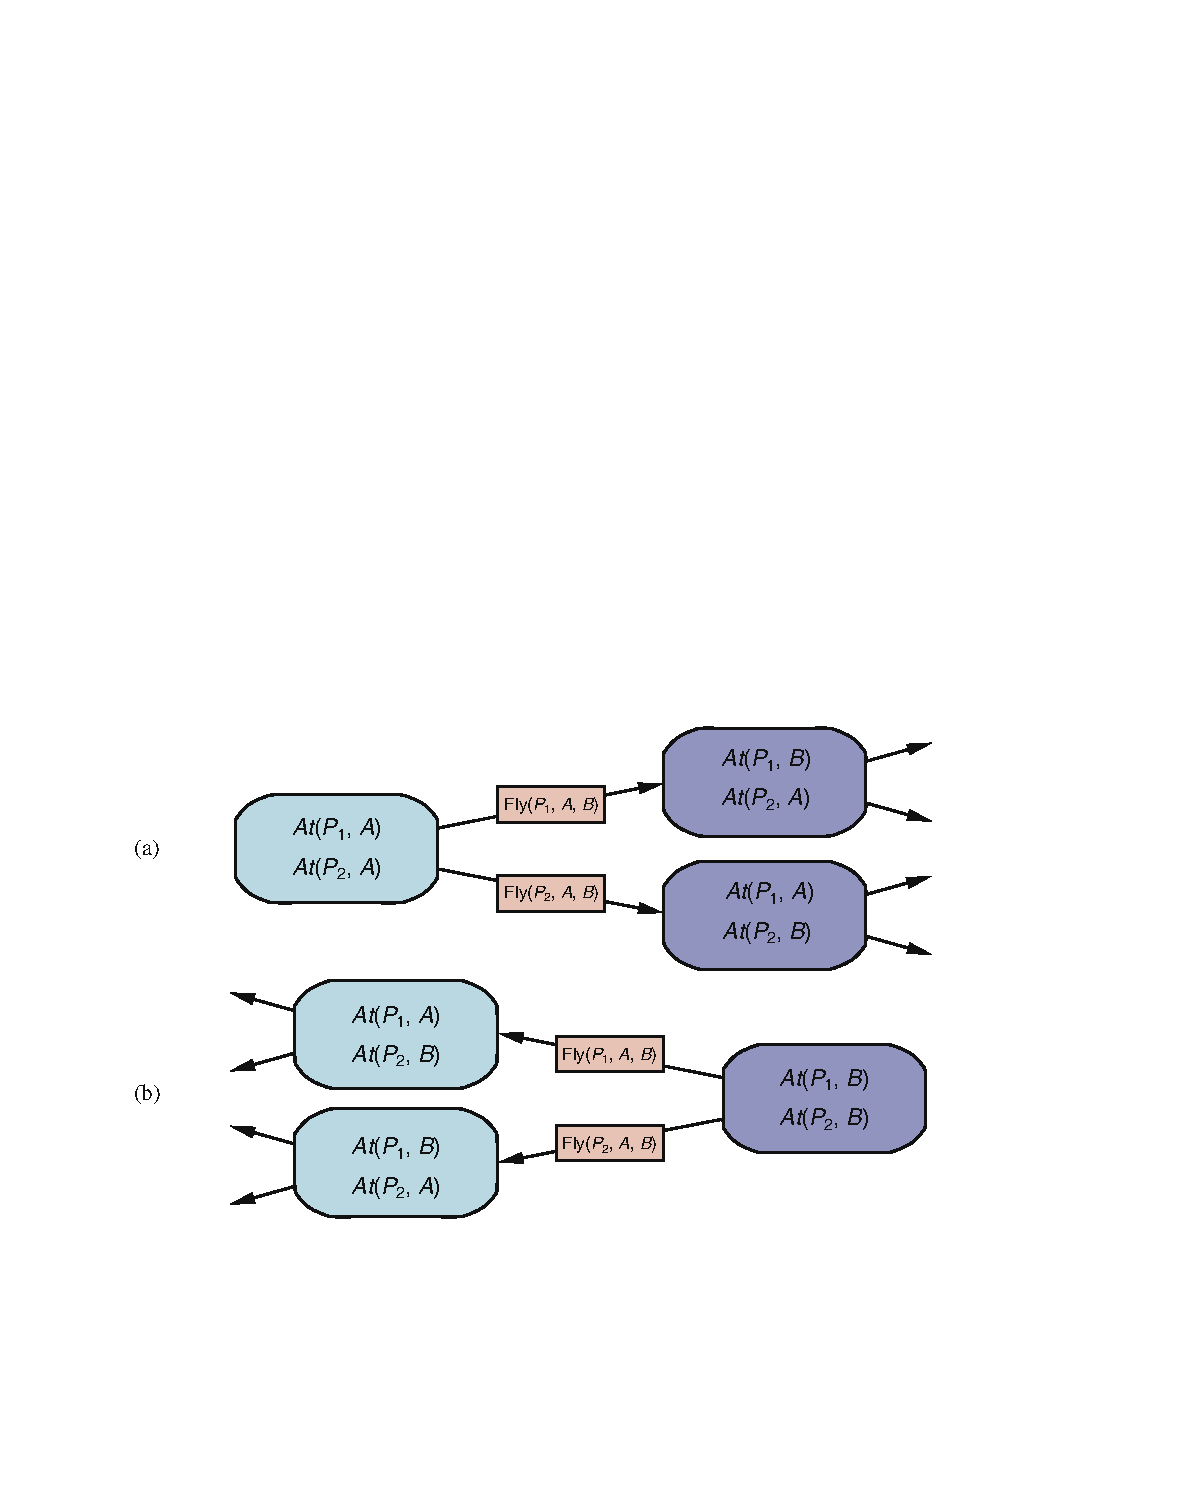
\includegraphics[alt={aima fig 11_05 forward backward search},height=2.4in]{aima-fig-11_05-forward-backward-search.pdf}
\section{Hierarchical Planning}
\label{sec:orgb78ffb4}




Hierarchical task network plans are built from:

\begin{itemize}
\item primitive actions, and
\item high-level actions (HLA).
\end{itemize}

HLAs have one or more \textbf{refinements}.

\begin{itemize}
\item Refinements may contain other HLAs.
\item A refinement with only primitive actions is an \textbf{implementation}.
\item An HLA achieves a goal if at least one of its implementations achieves the goal.
\end{itemize}





Here are two goal-achieving implementations for the \(Go(Home, SFO)\) HLA:


\vspace{.05in}
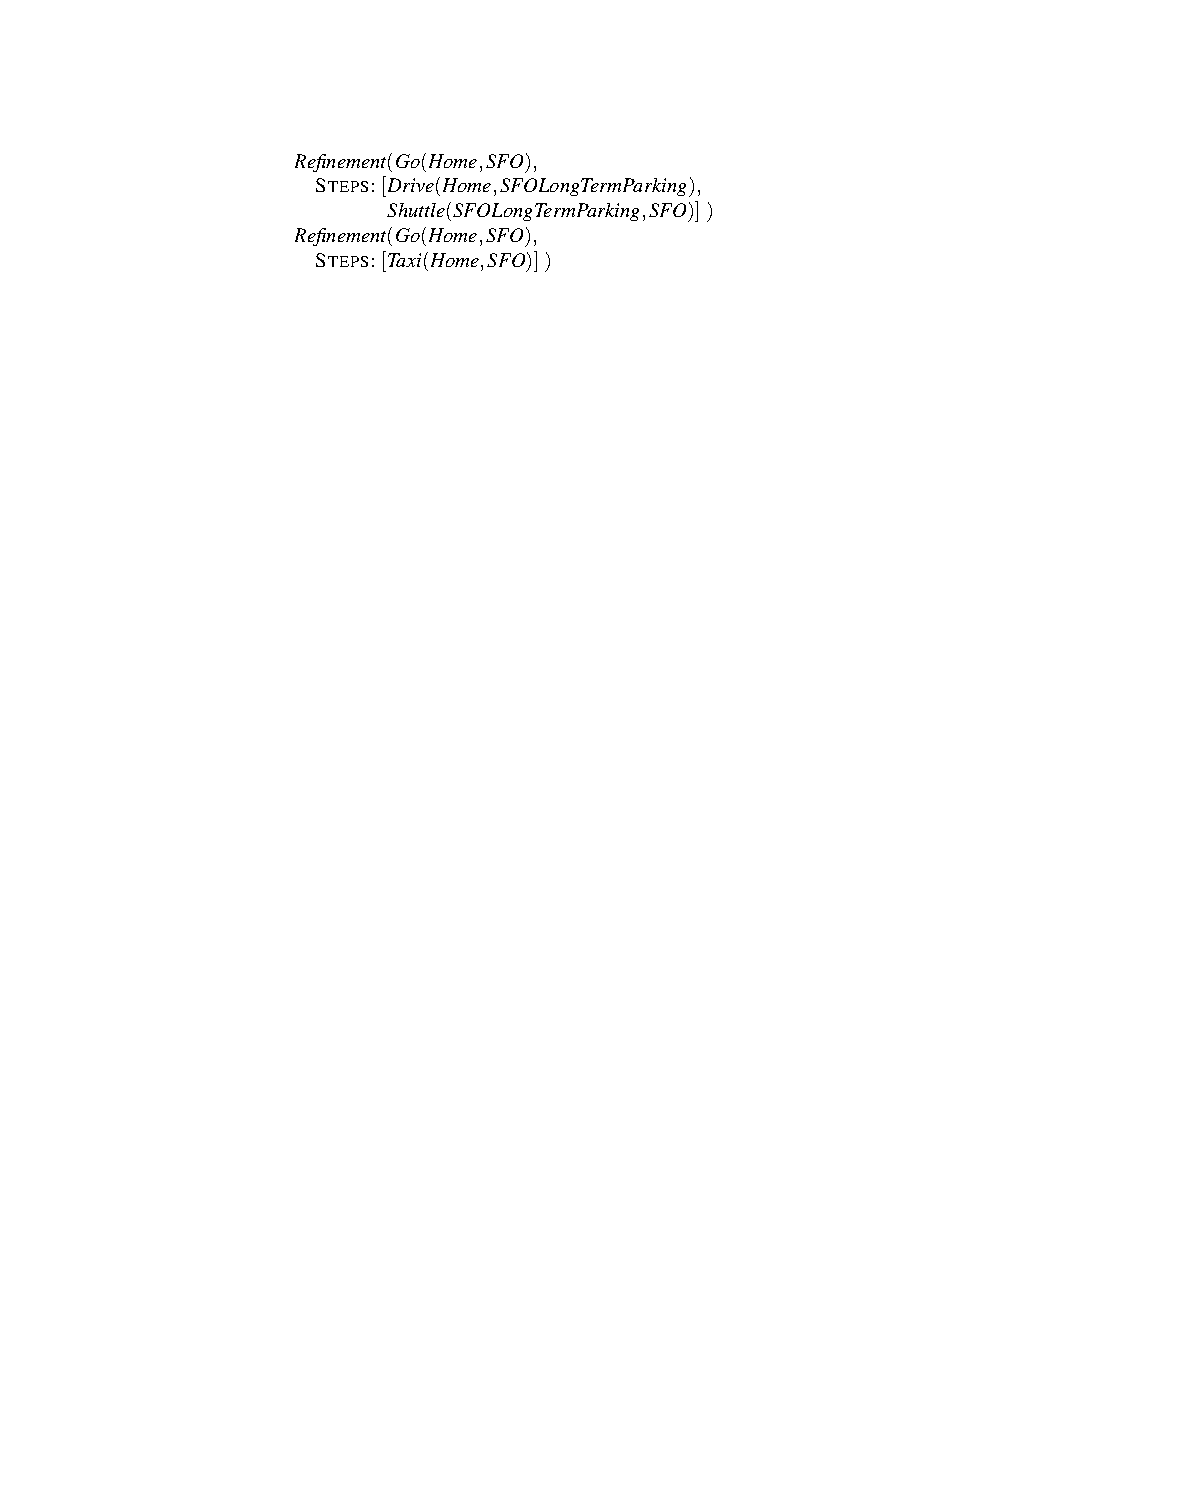
\includegraphics[alt={aima fig 11_07 a go home refinements},height=0.8in]{aima-fig-11_07-a-go-home-refinements.pdf}



Refinements can be produced recursivley, as shown in this vacuum world navigation example:


\vspace{.05in}
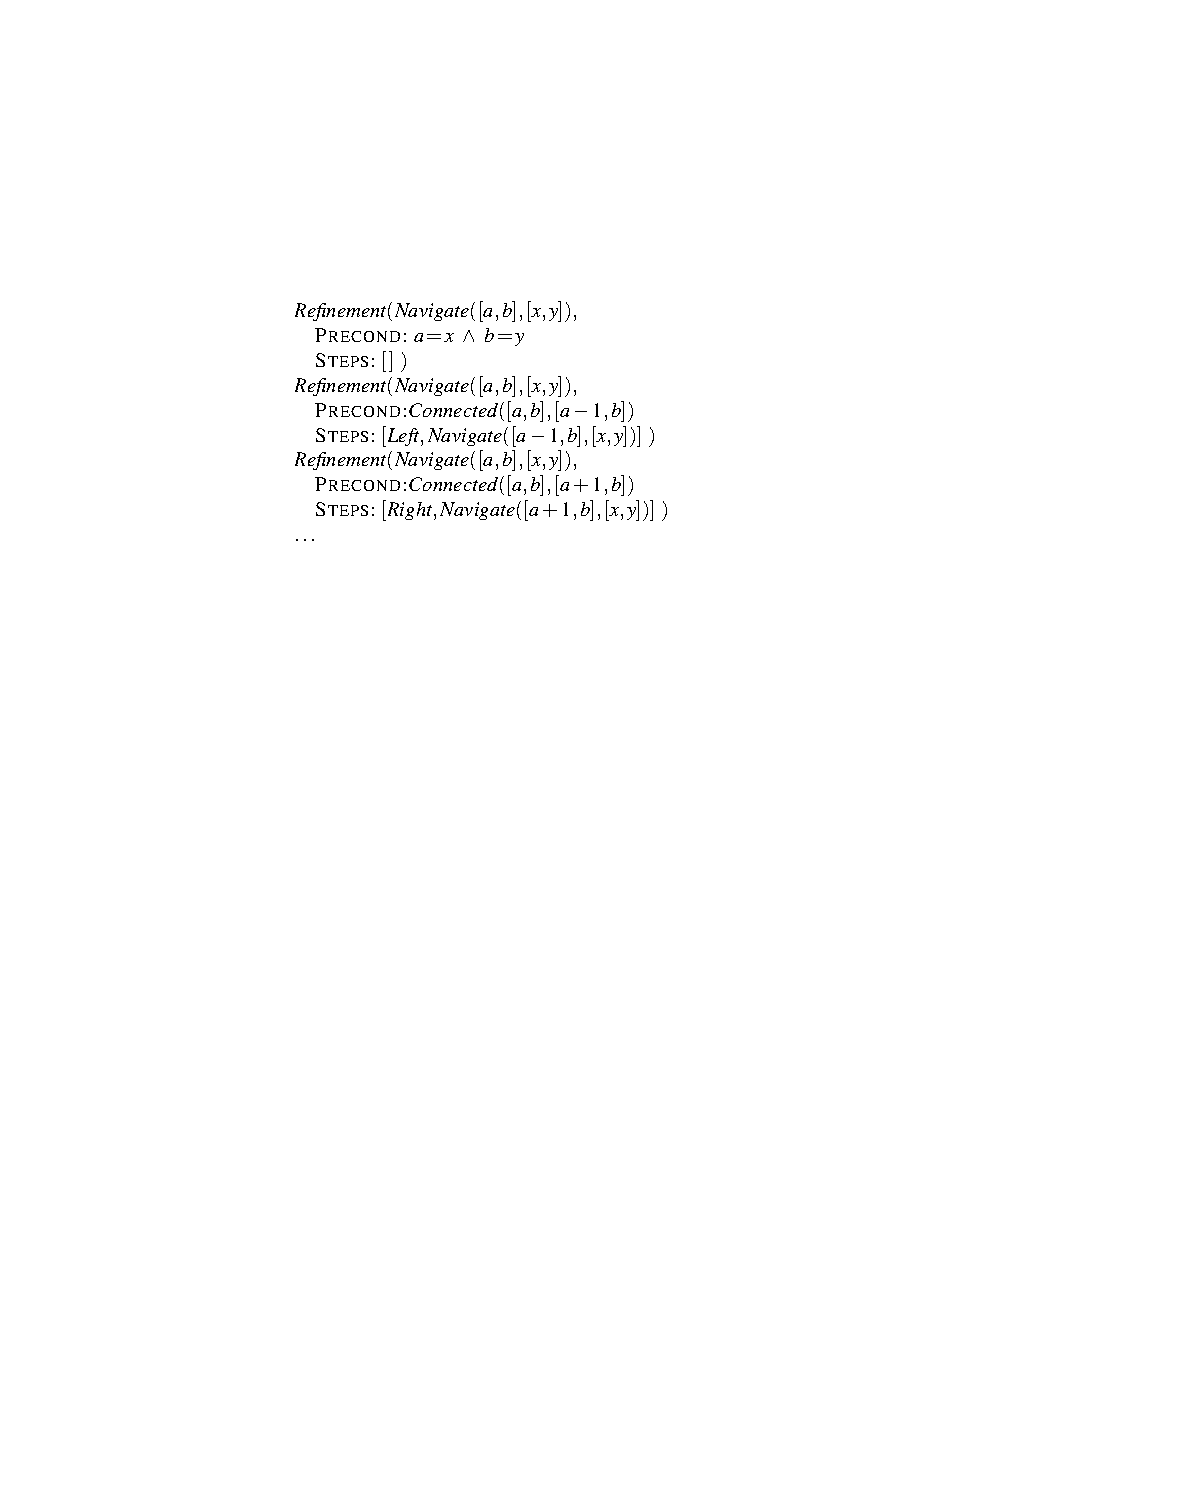
\includegraphics[alt={aima fig 11_07 b vacuum navigation recursion},height=1.6in]{aima-fig-11_07-b-vacuum-navigation-recursion.pdf}
\section{Closing Thoughts}
\label{sec:orgc77fb0c}

\begin{itemize}
\item Fun to create toy worlds and solve them.

\begin{itemize}
\item Look up "Monkey and bananas" problem.
\end{itemize}

\item Still have knowledge-acquisition bottleneck.
\item Still have problem of specifying large number of rules and facts for non-trivial problems.
\item Still have problem of uncertainty -- nondeterministic actions and partial observability.
\end{itemize}

In rest of course, we address these issues with uncertain reasoning and machine learning.
\end{document}
